\subsection{Within-Database Experiments}

\subsubsection{Finger Knuckle V3 Database with Deformation}

The Finger Knuckle V3 Database have 1-104 subjects that have two session samples, and the rest subjects of first session 105-221 just offer one session samples. So as the first experiment, I firstly fine-tuned my model on the second session of 1-104 subjects, and test on the first session 1-104 subjects. So it will have $104*6=624$ genuine matching scores, and have $104*103*6=64272$ imposter matching scores. From the below figure, if the false accept rate is below $10^{-2}$, the RFN-128-WRS is better than the RFN-128-WS. I also use the FKNet to train on this database, and the performance of FKNet is not better than the RFNet depend on the ROC figure. From the CMC and ROC, each model with WRS is better than WS on this dataset. For the ROC curve, I add EfficientNetV2-S model performance.

\begin{figure}[H]
	\centering
	\begin{subfigure}[b]{0.45\linewidth}
		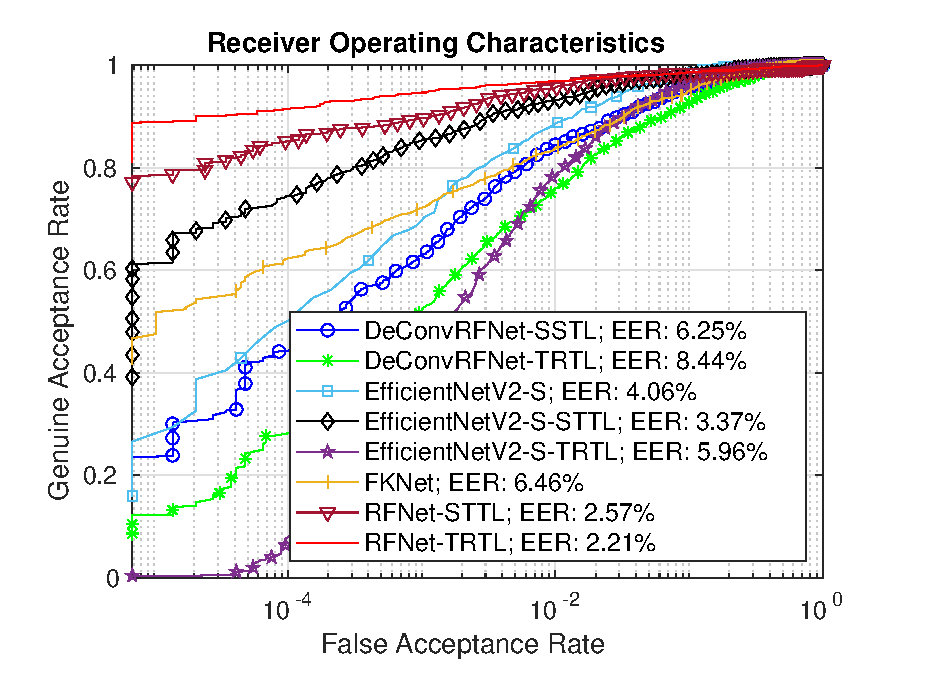
\includegraphics[width=\linewidth]{Figures/fkv3-roc_compare_new.eps}
	\end{subfigure}
	\begin{subfigure}[b]{0.45\linewidth}
		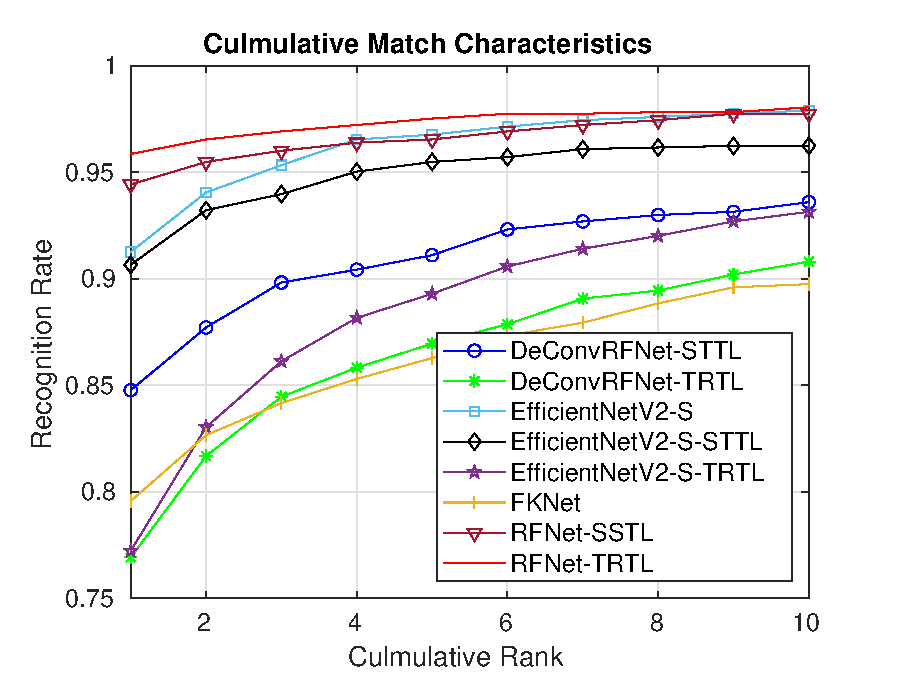
\includegraphics[width=\linewidth]{Figures/fkv3-cmc_compare_new.eps}
	\end{subfigure}
\end{figure}



As for the two-session protocol on the database. I should fine-tune my model on the 105-221 subjects, and use two-session protocol to evaluate my model performance on the 1-104 subjects dataset. In totally, it will generate $104*6=624$ genuine scores, and $104*103*6$ imposter scores. However, the FKNet is a classification task, and the output number classes should be same when training and testing. So the two session protocol experiment is not fit for FKNet. If the FKNet train on the 105-221 subjects and test on the 1-104 subjects with two sessions, the classes is different.

\begin{figure}[H]
    \centering
	\begin{subfigure}[b]{0.45\linewidth}
		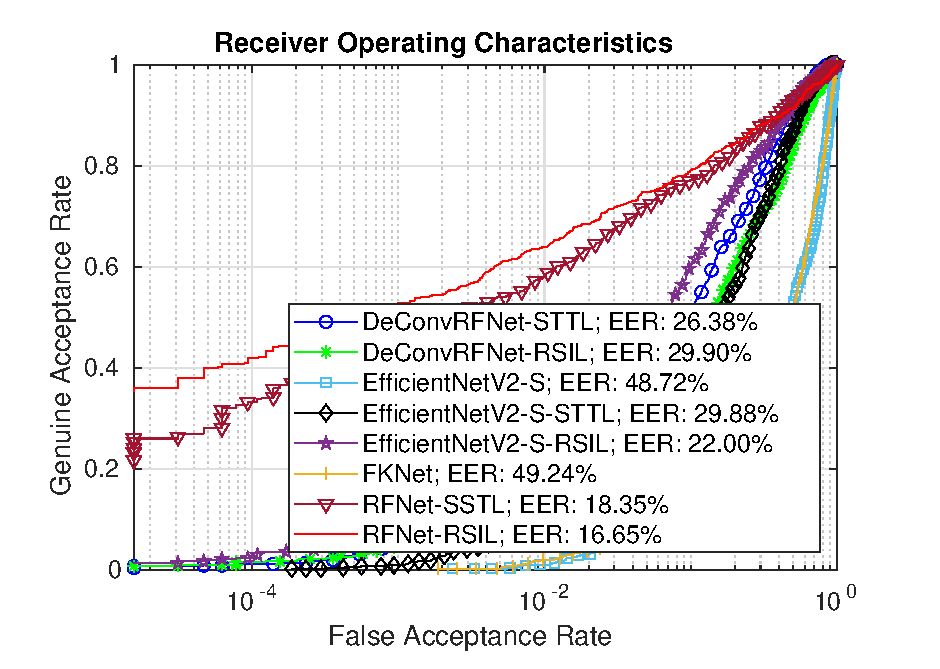
\includegraphics[width=\linewidth]{Figures/two-fkv3roc_compare_new.eps}
	\end{subfigure}
	\begin{subfigure}[b]{0.45\linewidth}
		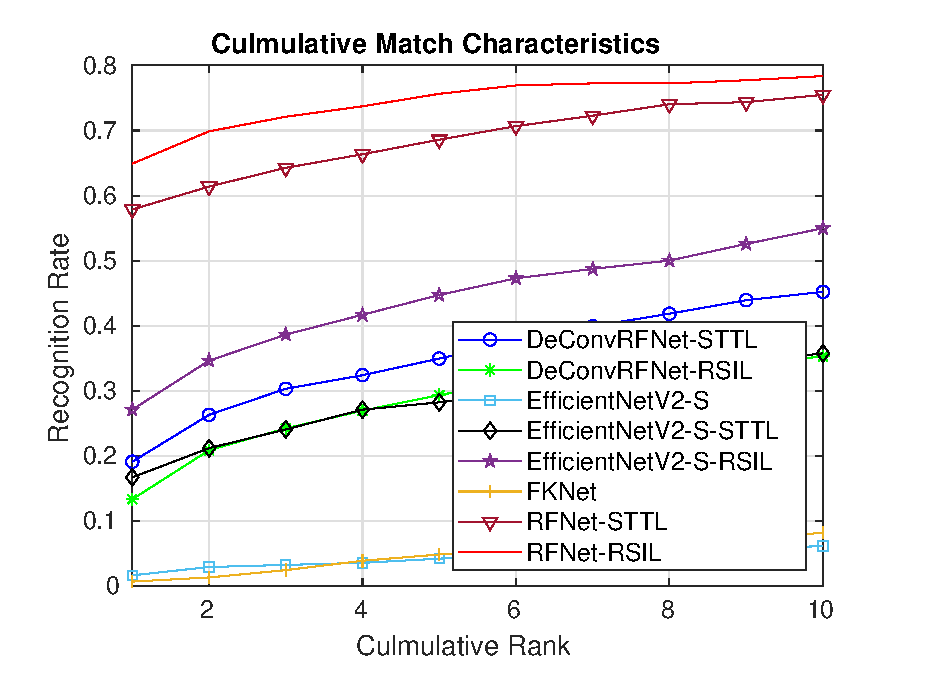
\includegraphics[width=\linewidth]{Figures/two-fkv3cmc_compare_new.eps}
	\end{subfigure}
\end{figure}

The two-session protocol will use the session1 as the probe and use the session2 as the enrollment. As for the genuine matching scores, each sample of a subject will choose the minimal matching score when compare to the rest samples. In this kind of situation, it will have $104x6$ genuine matching scores. Meanwhile, as for the imposter matching scores, it will also choose the minimal value result in $104*103*6$ imposter matching scores on the confusion matrix.

With Yolov5-CSL segmented finger knuckle, the RFNet performance is slightly higher than the local feature descriptors based on key points matching \cite{kumar2020contactless}, and performance higher than the paper \cite{kumar2019toward}. If we want to compare different method performance, I think we should use same dataset. In this kind of situation, the method of \cite{kumar2020contactless} maybe will get higher performance on the segmented finger knuckle by YOLOV5.

\subsubsection{Index Finger Knuckle of Hand Dorsal Image Database}
\begin{figure}[H]
	\centering
	\begin{subfigure}[b]{0.45\linewidth}
		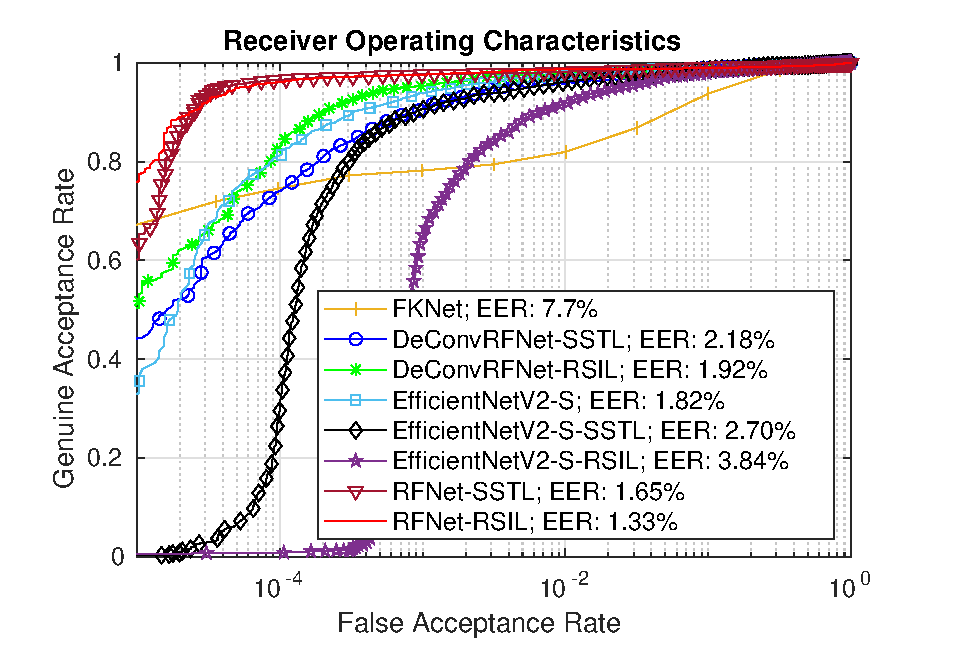
\includegraphics[width=\linewidth]{Figures/hd-roc_compare_new.eps}
	\end{subfigure}
	\begin{subfigure}[b]{0.45\linewidth}
		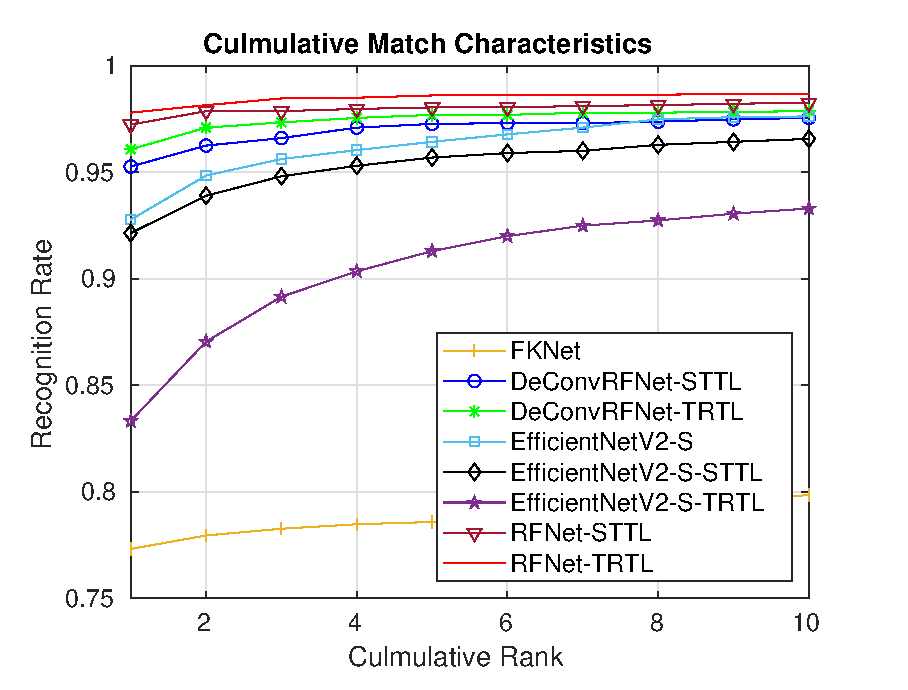
\includegraphics[width=\linewidth]{Figures/hd-cmc_compare_new.eps}
	\end{subfigure}
\end{figure}

As for the experiment, the dataset totally contains 712 subjects, and I use the segmented Index finger knuckle as my dataset. And I fine-tuned my model on the first sample of each subject, and then use the rest four sample as the testing dataset. At the testing process, it has $712*4=2848$ genuine matching scores, and has $712*711*4=2024928$ imposter matching scores. The performance of RFN-128-WRS and RFN-128-WS is similar, but the RFN-128-WS is slightly better than RFN-128-WRS depend on the EER value. And we can get an information that the RFNet is better than the rest network in the ROC figure, including the FKNet.


\subsubsection{2D Samples of 3D Finger Knuckle Database}

First experiment on the database is to use the one session 190 subjects image to fine-tune models and then to test on the another session 190 subjects. It has $190*6$ genuine matching scores and $190*189*6$ imposter matching scores. From the result, we can see that these RFN-128-WRS, RFN-128-WS, EfficientNetV2 can get very high matching accuracy. Meanwhile, the RFNet-TRTL has the minimal EER value among these models. As for the FKNet performance, it gets a very bad result on the 2D images of 3D finger knuckle. I think I have fully trained the FKNet. Maybe the model is overfitting on the training dataset.

\begin{figure}[H]
	\centering
	\begin{subfigure}[b]{0.45\linewidth}
		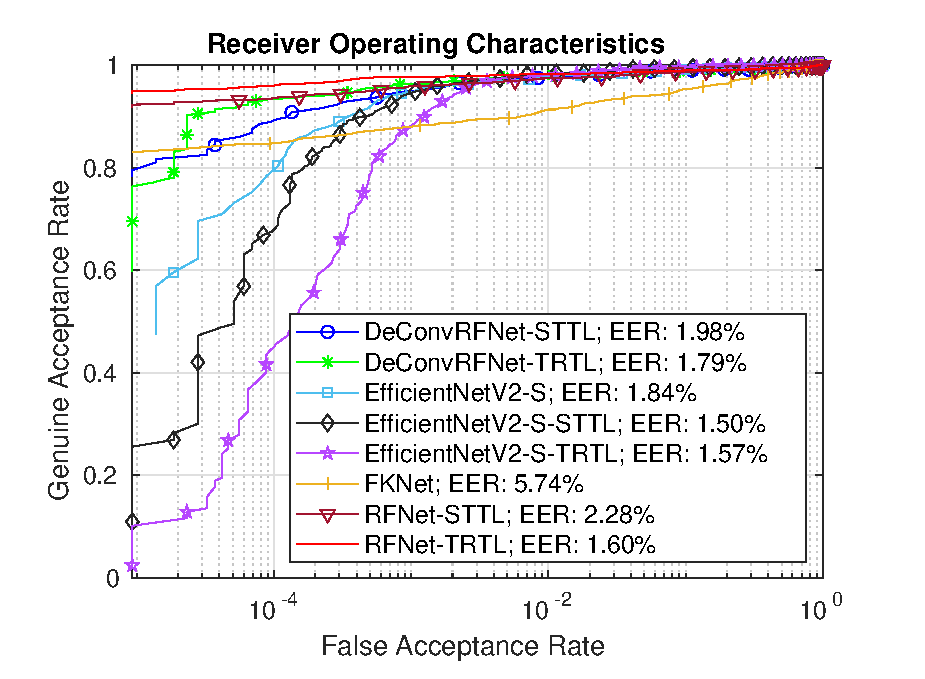
\includegraphics[width=\linewidth]{Figures/2dof3d-roc_compare_new.eps}
	\end{subfigure}
	\begin{subfigure}[b]{0.45\linewidth}
		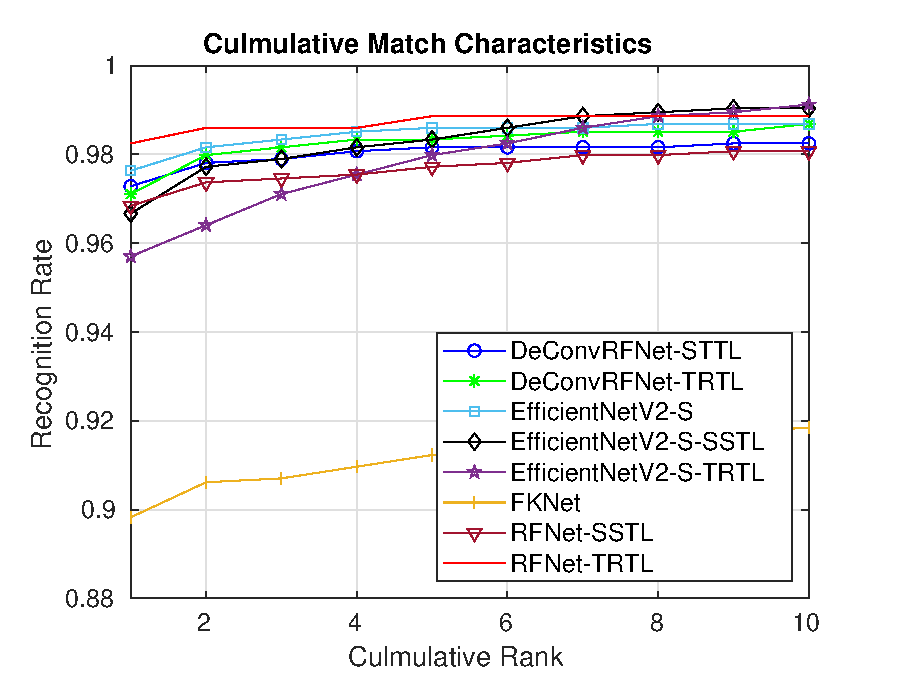
\includegraphics[width=\linewidth]{Figures/2dof3d-cmc_compare_new.eps}
	\end{subfigure}
\end{figure}


And then use the two session protocol. I use the rest samples of session1, and it has 191-228 subjects. In this kind of situation, the training dataset is too small. The two session protocol will test on the 190 subjects, these subjects can offer two session samples. Due to the training set is too small, so the matching performance is not very good. As for the FKNet, it cannot fit on two session protocol due to classification task.
